\documentclass [11pt, a4paper, oneside, article]{memoir}

%Inhaltsverzeichnis:
\usepackage{hyperref} %for hyperlinks
\maxtocdepth{section} %for depth in contents

%subsection numbering showed:
\setsecnumdepth{subsection}

%Including PDFs
\usepackage{pdfpages}

%Font: Arial
\usepackage{helvet}
\renewcommand{\familydefault}{\sfdefault}

% wenn unbekannte Silbentrennung dann in nächste zeile und große abstände
\sloppy

%Zeilenabstand:
\OnehalfSpacing

%Abstände zum Rand:
%TODO:
%\setlrmargins{1in}{*}{*}
%\setulmargins{0.6in}{0.6in}{*}

%Umlaute erlauben
%\usepackage[utf8]{inputenc

%Inserting Images:
\usepackage{graphicx}
\graphicspath{ {./images/} }

%For Highlighting Commands
\usepackage{listings}
\lstset{basicstyle=\tiny}

%Bibliography: APA
\usepackage{apacite}
\bibliographystyle{apacite}
% Change Caption language
\renewcommand{\figurename}{Abbildung}
\renewcommand{\figurerefname}{Abbildung}
\renewcommand{\contentsname}{Inhaltsverzeichnis}
%TODO: doesnt work:
\renewcommand{\bibname}{Literaturverzeichnis}


\begin{document}


\includegraphics[scale=0.07]{Logo_Uni-Kassel.png}\vspace{50pt}
\begin{center}
\textbf{Universität Kassel}\\
Fachbereich Maschinenbau\\\vspace{50pt}
\textbf{Portfolio}\\
Studiengang: Mechatronik\\\vspace{20pt}
\textbf{Fach: Wissenschaftliches Schreiben und Präsentieren für MechatronikerInnen}\\\vspace{50pt}

\begin{tabular}{rl}
Verfasser: & Johannes Hölker\\
 & Matr.-Nr. 35192059\\
 & Kattenstraße 9\\
 & 34119 Kassel\\
 & johannes.hoelker@uni-kassel.de\\\vspace{40pt}
 & \\
 & \\
 & Kassel, den 20. März 2021\\
\end{tabular}
\end{center}

\tableofcontents

\frontmatter
\chapter{Einleitung}
Diese Sammlung an Texten dient dem Bestehen des Kurses "Wissenschaftliches Schreiben und Präsentieren für Mechatronik", welcher im Wintersemester 2021/2022 von dem Verfasser belegt wurde.\\
Bei wöchentlichen Abgaben wurden Kenntnisse und Fähigkeiten im Verfassen wissenschaftlicher Texte und Arbeiten geübt und vertieft. Die entstandenen Aufsätze sind in überarbeiteter Version in diesem Portfolio zusammengefasst. \\
Die jeweiligen Rohversionen sind im Anhang zu finden, teils mit markierten Verbesserungen, welche in Partnerarbeit entstanden sind.\\
Die Inhalte der Texte befassen sich vorwiegend mit dem Klimawandel und der Frage, wie dieser mithilfe von unterschiedlichen Technologien und Aktionen auf ein bestimmtes Maß begrenzt werden kann. Dabei wird zum Beispiel über Elektromobilität und erneuerbare Energien gesprochen.\\
Des weiteren gibt es Aufsätze zu dem Studiengang Mechatronik und zu im Körper eingepflanzten Chips, eine Artikelrezension mit dem Thema Bewegung eines Roboterarms, eine Prozessgrafik zu einem Kaufprozess und abschließend eine Projektskizze zu einer Bachelorarbeit.
%TODO: was für BA


\mainmatter
\chapter{Hausaufgaben}
\section{HA 01: Warum sollte man Mechatronik studieren?}
  Computer, Auto, Smartphone, nahezu jedes Gerät aus deinem Alltag funktioniert so wie du es willst... Aber wie ist das möglich? Diese technischen Zusammenhänge zu erkennen und zu verstehen bringt der Studiengang Mechatronik mit sich.\\
  Im Grundstudium lernt man die Grundlagen aus den technischen Teilbereichen Maschinenbau, Elektrotechnik und Informatik kennen. Anschließend wird auf die Symbiose dieser Bereiche eingegangen und am Ende kann man sich nach den eigenen Interessen richten und sich spezialisieren. So werden dir im Laufe des Studiums die Abläufe vieler technischer Geräte und Prozesse klar.\\
  Dieses breit gefächerte Wissen ist nach abgeschlossenem Studium in deinem Repertoire und man hat anschließend die freie Wahl, auf welchen Fachbereich man sich nach dem Mechatronikstudium spezialisieren möchte oder ob man Schnittstellen der Fachbereiche koordiniert.\\
  Lass dir nach deinem Abitur nicht die Möglichkeiten nehmen und fokussiere   dich nicht zu früh auf einen Fachbereich, denn wer weiß welche Interessen du nach dem Studium haben wirst. Der Bachelor in Mechatronik qualifiziert dich für den Master in nahezu jedem technischen Zweig, sowie natürlich für einen Master in Mechatronik.\\
  Wenn deine Stärken in der Mathematik oder der Physik liegen bist du bei Mechatronik genau richtig. Aber auch wenn du nicht viel Vorerfahrung hast, kann der Studiengang Mechatronik was für dich sein. Du lernst die Grundlagen neu kennen und sie anschließend anwenden. Die Themen werden sehr grundsätzlich erklärt und mit dem nötigen Interesse kann man auch fachfremd in das Studium einsteigen.

\section{HA 02: Welche Technologie wird in den nächsten 5 Jahren von immenser Bedeutung sein?}
%„Überleitung von der Einleitung verbessern. Hier habe ich das gefühl das ich plötzlich reingeworfen werde “ zb Unsere welt wird häufiger von umweltkatasprophen heimgesucht , was auf die Erderwärmung zuruck zu führen ist....
  Um die Lebensgrundlagen der Menschheit und aller weiteren Tierarten nicht weiter zu gefährden und zu zerstören, darf die globale Erderwärmung keine 1,5° Celsius überschreiten \cite{masson-delmotte_ipcc_2019}.\\
  Um die schon jetzt auftretenden Folgen des anhaltenden Klimawandels noch stoppen zu können, kann an vielen unterschiedlichen Stellen etwas getan werden. Dazu gehört unter anderem der Verkehrssektor, der Ernährungssektor und vor allem der Energiesektor. Weltweit ist der Energiesektor der größte Emittent von Treibhausgasen, die Verbrennung fossiler Brennstoffe beträgt 88\% der CO2-Emmissionen, und das muss sich zwangsläufig und innerhalb kurzer Zeit ändern \cite{quaschning_regenerative_2019}.\\
  Die nötigen Mittel das zu erreichen haben die Menschen schon erfunden. Mit Solar- und Winkraftanlagen gibt es zwei ausgereifte Technologien, welche saubere Energie liefern. Diese Energieproduzenten können in Deutschland, sowie auf der ganzen Welt errichtet werden. \\
  Jedes Hausdach kann potenziell ein Solarkraftwerk werden. Deshalb sollte bei Neubauten auf eine Abdeckung mit Solarplatten geachtet werden. Die Technologie ist insofern ausgereift, dass die aktuell zum Verkauf stehenden Solarplatten technisch nicht mehr verbessert werden können. Lediglich eine thermische Nutzung mit Wasser kann den Wirkungsgrad noch erhöhen. Das erwärmte Wasser kann dann für die Heizung oder das Warmwasser genutzt werden.\\
  Noch nicht ausgereift ist die Energiespeicherung. Diese ist essentiell für eine erfolgreiche Energiewende. Das bedeutet, dass unsere Nutzung von Energie sich zwangsläufig an die Energiegenerierung anpassen muss. Nur wenn die Sonne scheint und der Wind weht, wird Energie generiert und bei einem Überschuss werden die Akkus geladen. Wenn diese irgendwann leer sein sollten, kann auch keine Energie mehr bezogen werden.\\
  Ein großer Vorteil der Technologie Solar ist die Möglichkeit der dezentralen Verteilung. Mit einem weit verbeiteten Netz aus vielen Akkus, welche sich dann gegenseitig unterstützen, kann trotzdem eine durchgehende Versorgung gewährleistet werden. Erst durch die polyzentral verteilte Generierung und Speicherung von Solarstrom, welche durch Batteriestationen in jedem Haus erreicht wird, können wir unabhängig von fossilen Energieträgern werden.\\
  %"Unabhängig werden" ist dabei ein zentraler Begriff. Ohne die Verlegung von langen Leitungen kann ein Haushalt in der Peripherie mit einer sogenannten Inselnetzanlage autark mit Strom versorgt werden.
  %An das Netz gekoppelte Systeme dagegen bekommen den überschüssigen Strom ausbezahlt, das macht einen Hausbesitzer/ eine Hausbesitzerin mit großer Dachfläche zu einem Energielieferanten und im besten Fall kann man davon sogar leben.

\include{Hausaufgaben/3_Elektromobilitaet/Elektromobilität_Johannes}
\section{HA 09: Projektskizze einer Abschlussarbeit}
\subsection{Deckblatt}

\includegraphics[scale=0.07]{Logo_Uni-Kassel.png}\vspace{50pt}
\begin{center}
\textbf{Universität Kassel}\\
Fachbereich Maschinenbau\\
Arbeits- und Organisationspsychologie\\\vspace{50pt}
\textbf{Bachelorarbeit}\\
Mechatronik\\\vspace{20pt}
\textbf{Intuitive Telepräsenzsteuerung eines anthropomorphen Manipulators unter Verwendung von Head-Mounted Displays und Motion-Capturing}\\\vspace{30pt}
\begin{tabular}{rl}
Betreuer: & Prof. Dr. phil. habil. Oliver Sträter\\
 & Dipl. Ing. M.Sc. Mehrach Saki \\
  & \\
Verfasser: & Johannes Hölker\\
 & Matr.-Nr. 35192059\\
 & Kattenstraße 9\\
 & 34119 Kassel\\
 & johannes.hoelker@uni-kassel.de\\\vspace{40pt}
 & \\
 & \\
 & Kassel, den 20. März 2021\\
\end{tabular}
\end{center}

\subsection{Gliederung}
0 Abstract

1 Introduction [Argumentation]
  1.1 Motivation (Relevance of the topic)
  1.2 Aim of the thesis
  1.3 Aufbau der Arbeit

2 Theory (What is necessary to know for this work to read?) [Beschreibung]
  2.1 Robotics
    2.1.1 Manipulator
    2.1.2 Controlling
    2.1.3 Kinematics
    2.1.4 ..
  2.2 Teleoperation
    2.2.1 Camerasystem (Monitor)
    2.2.1 Vr glasses
  2.3 Data stream
    2.3.1 transfer rate
  2.4 Research question

3 Methods [Argumentation/Beschreibung]
  3.1 Mocap (Motion Tracking)
  3.2 Stitching onto VR-glasses
  3.3 Robot system (ROS)

4 Concept [Argumentation/Beschreibung]
  What is the idea? (VR+Mocap+360°+Position)

5 Realization (Development - How did I build the system?) [Argumentation/Beschreibung]
  5.1 Controlling the robot (ROS) -> Code
  5.2 Image Transmission (360 + Stereostitch)
  5.3 Mounting / Position of the camera

6 Function Validation (Is the system working as aspected?) [Argumentation/Beschreibung]

7 Discussion and Outlook [Argumentation]

8 References

\section{Fragestellung}
%Wird einem potenziellen Betreuer ersichtlich, woran ich forschen möchte?
%Sind meine Ausführungen überzeugend und helfen sie, mein Thema zu "verkaufen"?
%Problemstellung:
  Die Programmierung und Steuerung von Manipulatoren geschieht aktuell noch über ein Umdenken des Anwenders indem er von einer anderen Perspektive auf das System schaut und es so steuert. Das kann Komplikationen erzeugen, erfordert Einarbeitung und Erfahrung und macht die Werkzeugtransformation schwierig. Um die fortschreitende Automatisierung für eine breite Masse verfügbar zu machen, müssen Manipulatoren intuitiv bedienbar sein. \\
%Zielsetzung:
  Ein System, was die Technologien der Robotik und der Datenbrillen kombiniert, kann helfen diese Problematik zu lösen. Durch Einsatz von Telepräsenz soll die anwendende Person die Perspektive des Roboters einnehmen und den Roboterarm intuitiv steuern können. \\
%Forschungsfrage:
  Die in dieser Arbeit behandelte Forschungsfrage lautet demnach:
  Wie lässt sich ein System mit den beiden Technologien Robotik und Datenbrillen bauen, um funktionierende Telepräsenz zu erreichen und so eine intuitive Steuerung eines Manipulators zu ermöglichen?

\subsection{Textprobe: vorläufige Einleitung}
%Ist der Text verständlich?
%Einhaltung sprachlicher und formaler Standards
  Zu Beginn dieser Arbeit wird die Motivation erläutert, aus welcher diese heraus geschrieben wird. Anschließend leitet sich daraus die Zielstellung ab und ein Überblick über die folgenden Kapitel wird präsentiert.
\subsubsection{Motivation}%Warum möchte ich das erforschen?
  Der erste ferngesteuerte Roboter, 1949 erfunden von Raymond Goertz, wurde dazu eingesetzt radioaktives Material gefahrenfrei zu bewegen. Die eingesetzte Methode des Master-Slave Manipulators übersetzte mechanisch die Bewegung des menschlichen Arms auf einen Manipulator. So konnten Gefahrengüter hinter einer durchsichtigen Trennwand bewegt werden. Dabei merkte Goertz an, dass die anwendende Person aus einem anderen Blickwinkel auf die auszuführende Aufgabe schauen muss und die Aufgabe so erschwert wird \cite{goertz_master-slave_1949}. \\\\
  Diese Problematik ist in der Robotik größtenteils durch eine Automatisierung der Manipulatoren gelöst worden. Durch ein hohes Maß an Sensorik und in kürzester Vergangenheit auch durch den Einsatz neuronaler Netze können sich Roboter weitgehend selbstständig bewegen \cite{siciliano_springer_2008}.\\\\
  % Ausführung von für den Menschen gemachten Arbeitsaufgaben
  Es gibt jedoch weiterhin viele Aufgaben, bei denen ein Mensch anwesend sein muss. Die Wartung von industriellen Maschinen, Pflegetätigkeiten und kooperatives Arbeiten sind nur ein paar Beispiele. Viele Arbeitsumgebungen sind des Weiteren für den Menschen konzipiert und die Aufgaben sind komplex und damit nicht direkt automatisierbar \cite{fritsche_first-person_2015}. Um dennoch die Aufgaben lösen zu können, ohne dass ein Mensch anwesend ist, kann ein anthropomorpher ferngesteuerter Manipulator eingesetzt werden \cite{tanie_mfi_2003}\cite{stanczyk_development_2006}.\\\\
  Herkömmliche Programmierverfahren erfordern des Weiteren viel Übung und Zeitaufwand. Die programmierende Person muss eine spezielle Ausbildung haben und braucht dennoch gewisse Zeit für die Umsetzung. Besonders in kleinen und mittelständischen Unternehmen bringen günstige Robotersysteme, welche einfach zu installieren, einzustellen, zu programmieren und zu warten sind, einen Vorteil. Um die genannten Arbeitsschritte zu vereinfachen erfordert es eine intuitive Steuerung des Roboters \cite[S.76]{brogardh_present_2007} \cite[S.190]{ehlers_echtzeitfahige_2019}. \\\\
  Räumlich in die Rolle des Roboters zu schlüpfen und aus der veränderten Perspektive heraus zu handeln eignet sich für eine Manipulatorsteuerung in für Menschen gefährlichen Umgebungen \cite[S.9]{mareczek_grundlagen_2020}. Diverse Konzepte und Systeme um diese Problematik zu lösen wurden entwickelt und werden in Kapitel 2 vorgestellt.\\\\
  % Mensch vor Technik:
  In der vorliegenden Arbeit wird demnach ein Arbeitsplatz gestaltet, welcher den Menschen mit Technik verbindet. Es werden Geräte eingesetzt, welche der Mensch tragen soll und so sein Umfeld beeinflussen. Für die gesamte Arbeitsgestaltung ist dabei wesentlich, dass nicht die technische Machbarkeit, sondern die "menschlichen Bedarfe und Möglichkeiten" im Vordergrund stehen \cite{strater_positionspapier_2019}. Für alle Entwicklungsschritte wird diese Richtlinie bedacht und evaluiert.\\\\
  % OpenSource für Nachhaltigkeit
  Aufgrund der aktuellen Situation des globalen Klimas \cite{ipcc_climate_2021}, soll die technische Entwicklung auch in Hinblick auf Nachhaltigkeit geschehen. Der Einsatz von Open Source Design (OSD) kann nach \cite{setchi_implications_2016} während und zum Ende des Lebenszyklus eines technischen Produkts einen positiven Einfluss auf Nachhaltigkeit haben. Die Reparierbarkeit, Wiederverwendbarkeit und die lokal-gebundene Wertschöpfung werden durch Ntzung von OSD ermöglicht und haben damit eine erhöhte Effizienz bei der Ressourcennutzung.
\subsubsection{Zielstellung} \label{1:sec:ziel}
  An die bereits bestehenden Konzepte soll diese Arbeit anknüpfen und die Entwicklung eines immersiven Systems zur Manipulatorsteuerung wird präsentiert. Die nutzende Person soll möglichst intuitiv einen Manipulator steuern können, ohne dass Vorerfahrung vorhanden ist. Dabei lautet das zentrale Ziel, die nutzende Person visuell in die Rolle des Roboters schlüpfen zu lassen. \\\\
  Um dies zu erreichen wird mit den Technologien Motion-Capturing und Head-Mounted Displays (HMD) gearbeitet. Bei der Entwicklung des Manipulators wird soweit möglich mit OSD gearbeitet, in diesem Fall bedeutet dies den Einsatz von 3D-Druck und die Nutzung des Robot Operating Systems (ROS). Bei der gesamten Entwicklung soll des Weiteren ein auf den Menschen zugeschnittenes System entwicklet werden, wobei nicht die technische Machbarkeit im Vordergrund steht.
\subsubsection{Aufbau der Arbeit}
  Nachdem nun die Hintergründe für die Entstehung dieser Arbeit erläutert wurden, werden zunächst die für das Verstehen der Arbeit nötigen wissenschaftlichen Erkenntnisse in Kapitel 2 zusammengefasst. Der Begriff und die Erreichung von Telepräsenz wird in Kapitel 2 erläutert, sowie die Grundlagen für Manipulatoren in Kapitel 2 gegeben\\
  In Kapitel Kapitel 3 werden die eingesetzten Methoden erklärt. Die der Umsetzung zugrundeliegende Konzeptidee wird in Kapitel 4 präsentiert und erläutert.\\
  Anschließend wird auf das Vorgehen bei der Realisierung des Konzepts in Kapitel 5 eingangen und aufgetretene Problematiken werden benannt.\\
  Das entstandene System wird in Kapitel 6 auf die Funktion hin geprüft und validiert. Die benannten Problematiken und Schwierigkeiten bei der Umsetzung werden in Kapitel 7 diskutiert und ein Ausblick auf die zukünftige Forschung wird gegeben.\\

\section{Projektablaufplan}
%Realisitsch und nachvollziehbar?

%TODO: include bib für BA
\subsection{Inhaltsverzeichnis}
%\bibliography{bibs/01_Intro.bib}


\chapter{Fazit/Reflexion}
In dem vorliegenden Portfolio wurde auf diverse Themen eingegangen, welche sich einerseits mit Technologien und andererseits mit dem Umgang des Menschen mit der Natur und dem Klimawandel beschäftigen. Dabei wurde zu Beginn die Frage gestellt, ob der menschengemachte Klimawandel noch begrenzt werden kann. Diese Frage wurde in den vorliegenden Aufsätzen nicht abschließend geklärt. Dies ist aufgrund der Komplexität des Themas aber auch nicht in diesem Umfang möglich oder wurde nicht angestrebt. Es wurden Lösungsansätze aufgezeigt und Fakten gesammelt, welche das Problem angehen und beziffern.\\\\
Es sei des Weiteren angemerkt, dass, wie in \ref{ha04} schon angemerkt, nicht nur der Energiesektor und die neuen Technologien eine Rolle spielen. Auch die Nahrungsmittelproduktion trägt mit knapp einem fünftel zu der Treibhausgasproduktion bei. Und gerade hier können die Aktionen eines jeden Einzelnen eine Rolle spielen. Mit jeder Entscheidung anstatt eines tierischen ein rein pflanzliches Produkt zu kaufen und zu essen, kann ein Einfluss auf den fortschreitenden Klimawandel genommen werden \cite{poore_reducing_2018}. Auch wenn die Hilflosigkeit über den geringen eigenen Einfluss auf große Probleme erdrückend ist, basiert die zukünftige Welt und Umwelt auf den eigenen zu jedem Zeitpunkt getroffenen Entscheidungen.

%\refstepcounter{chapter}
%\addcontentsline{toc}{ chapter }{\ bibname}
\bibliography{bibs/BA_final.bib}

%TODO: include raw documents im Anhang
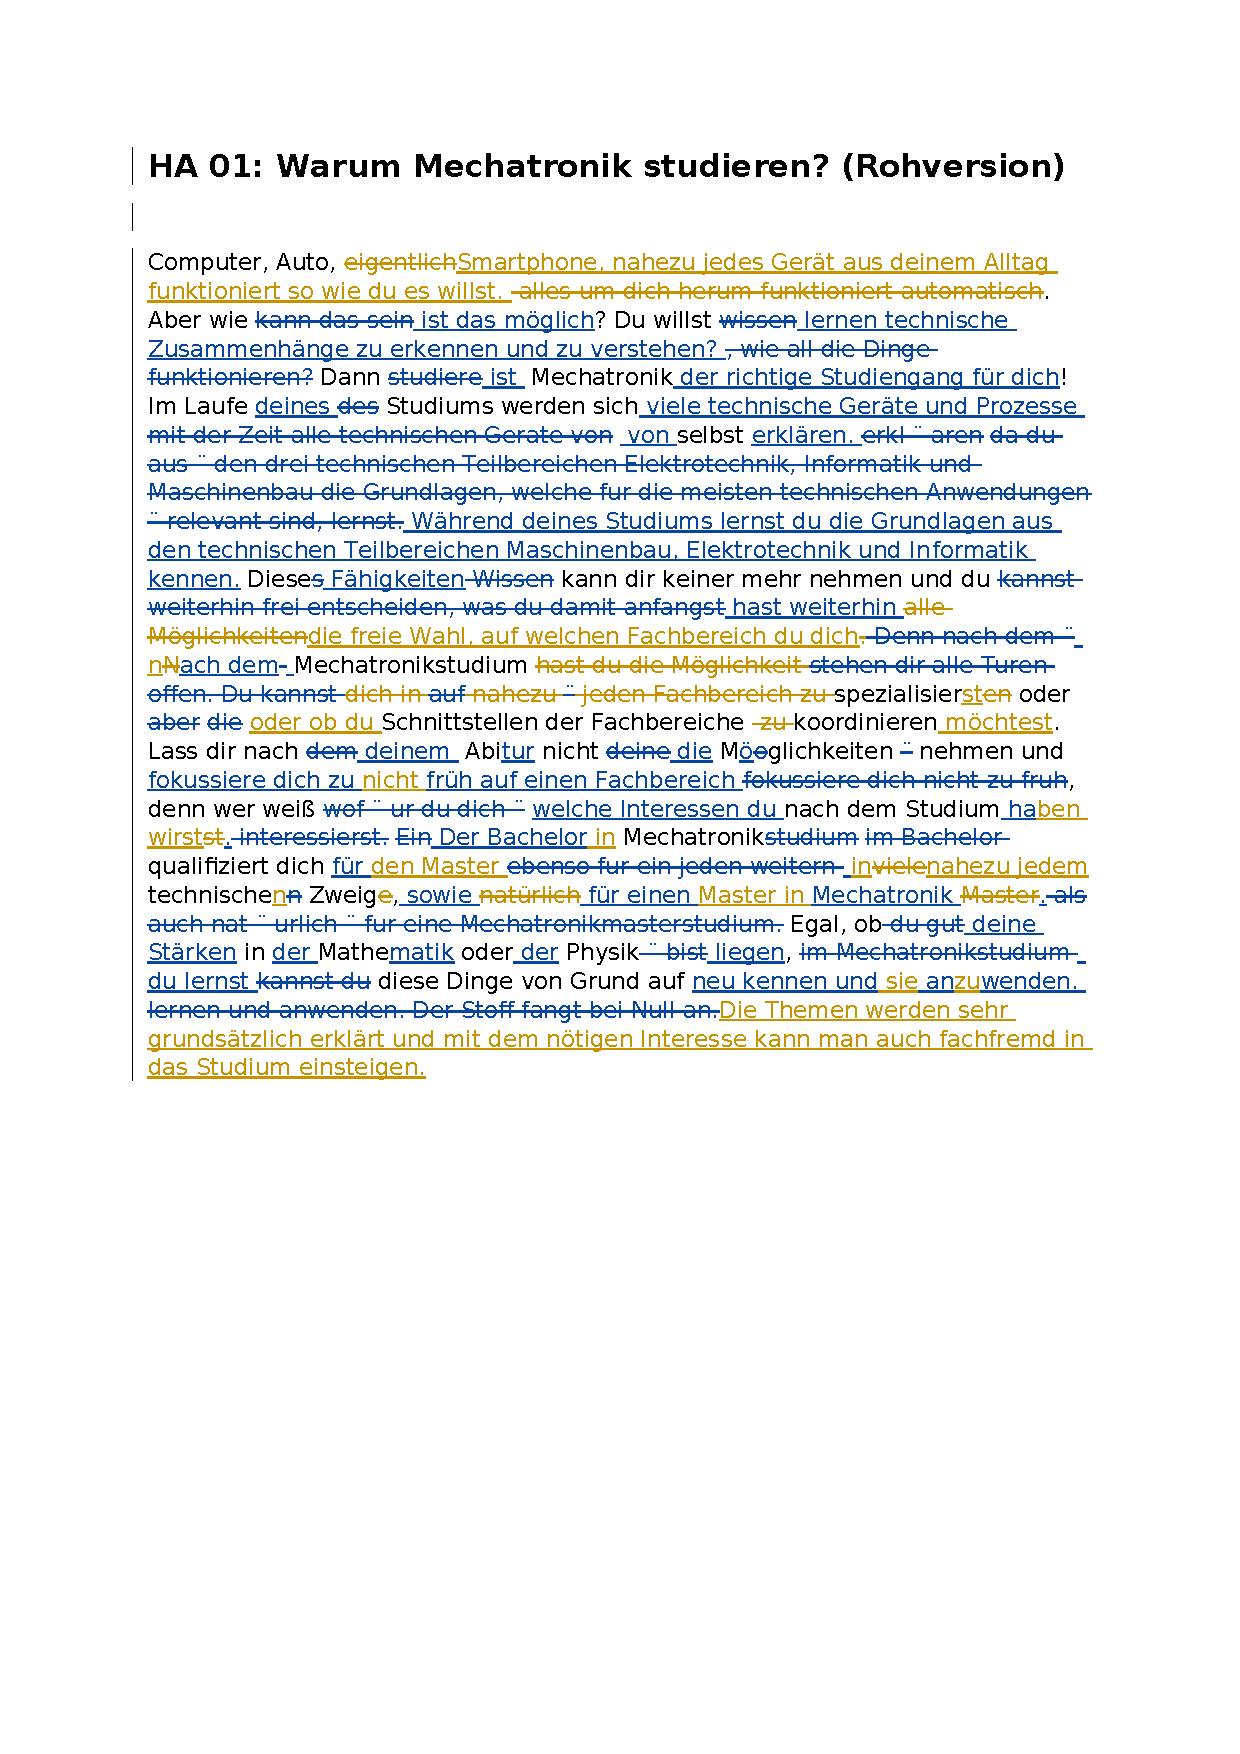
\includepdf[pages=-]{./Hausaufgaben/1_Warum_Mechatronik_studieren/Warum_Mechatronik_Johannes_Rohversion.pdf}
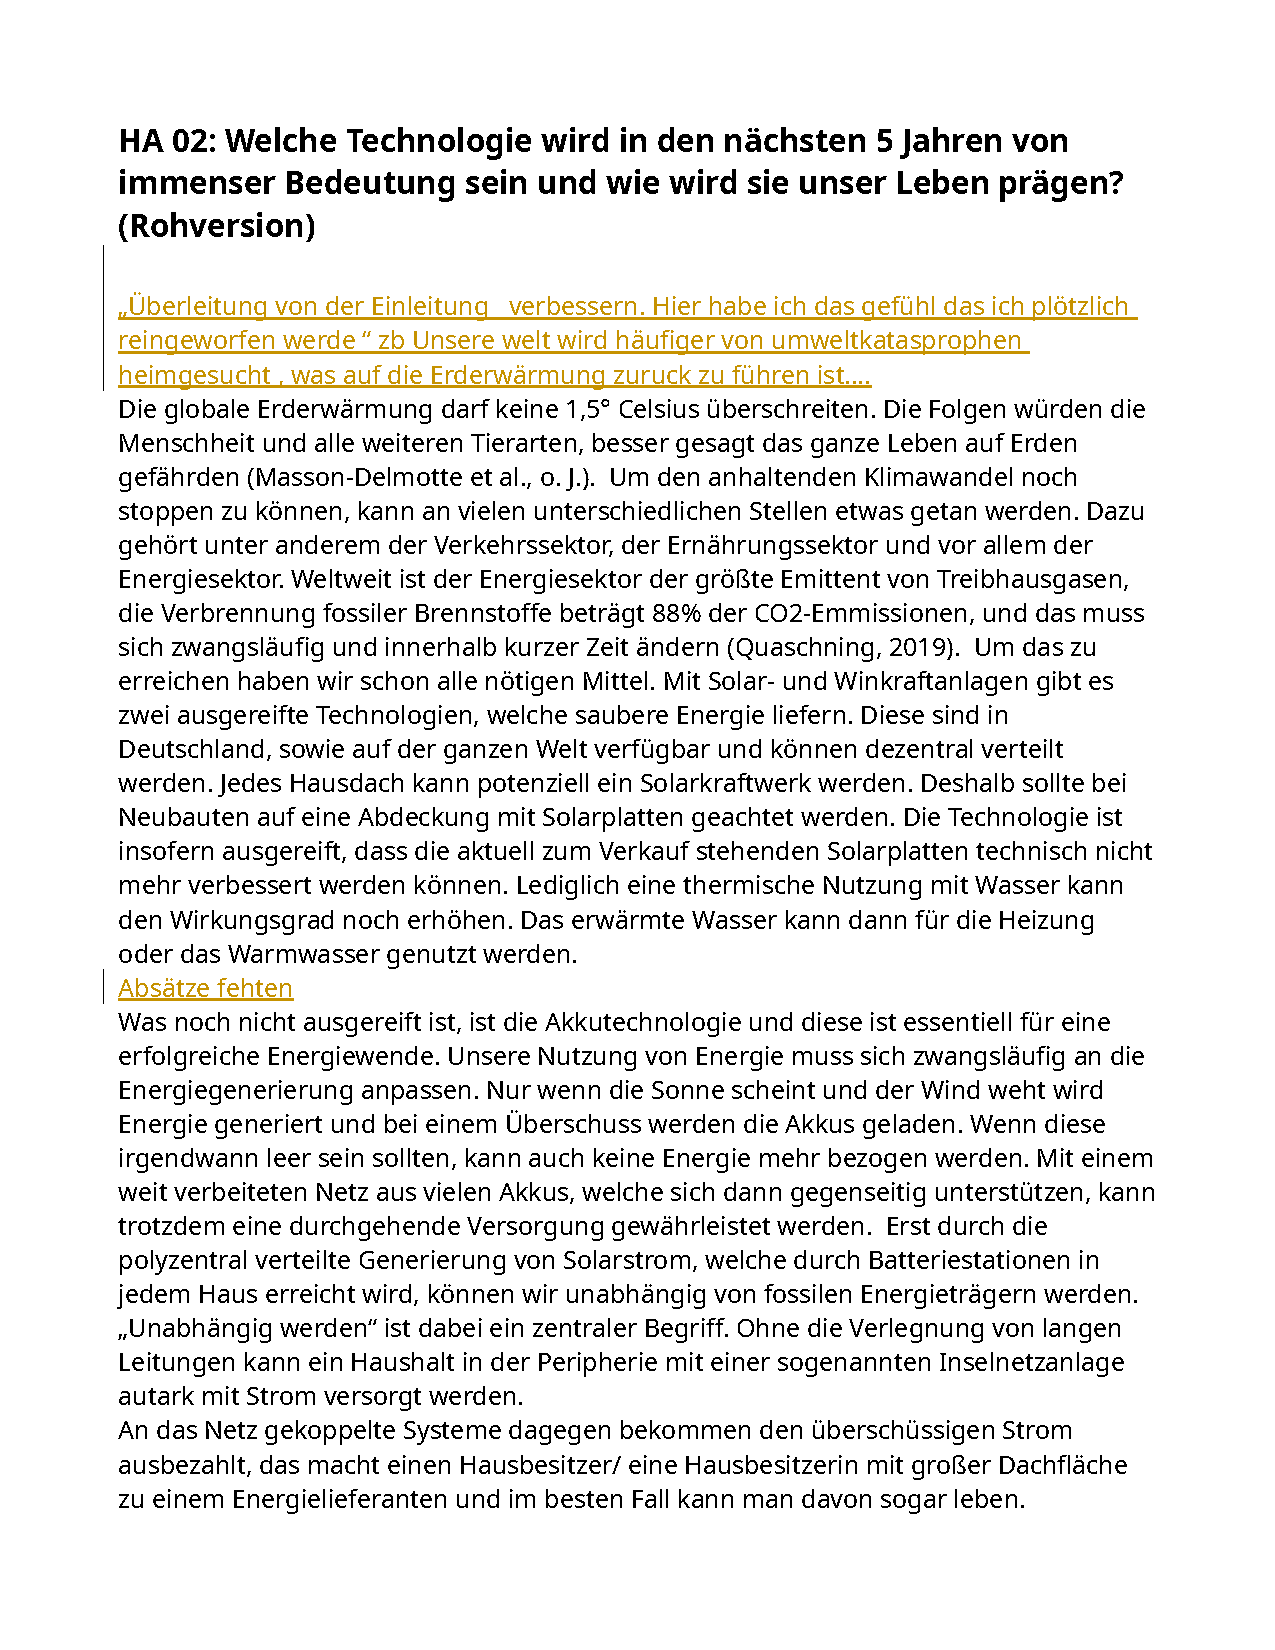
\includepdf[pages=-]{./Hausaufgaben/2_Zukunftstechnologie/Technologie_Johannes_Rohversion.pdf}
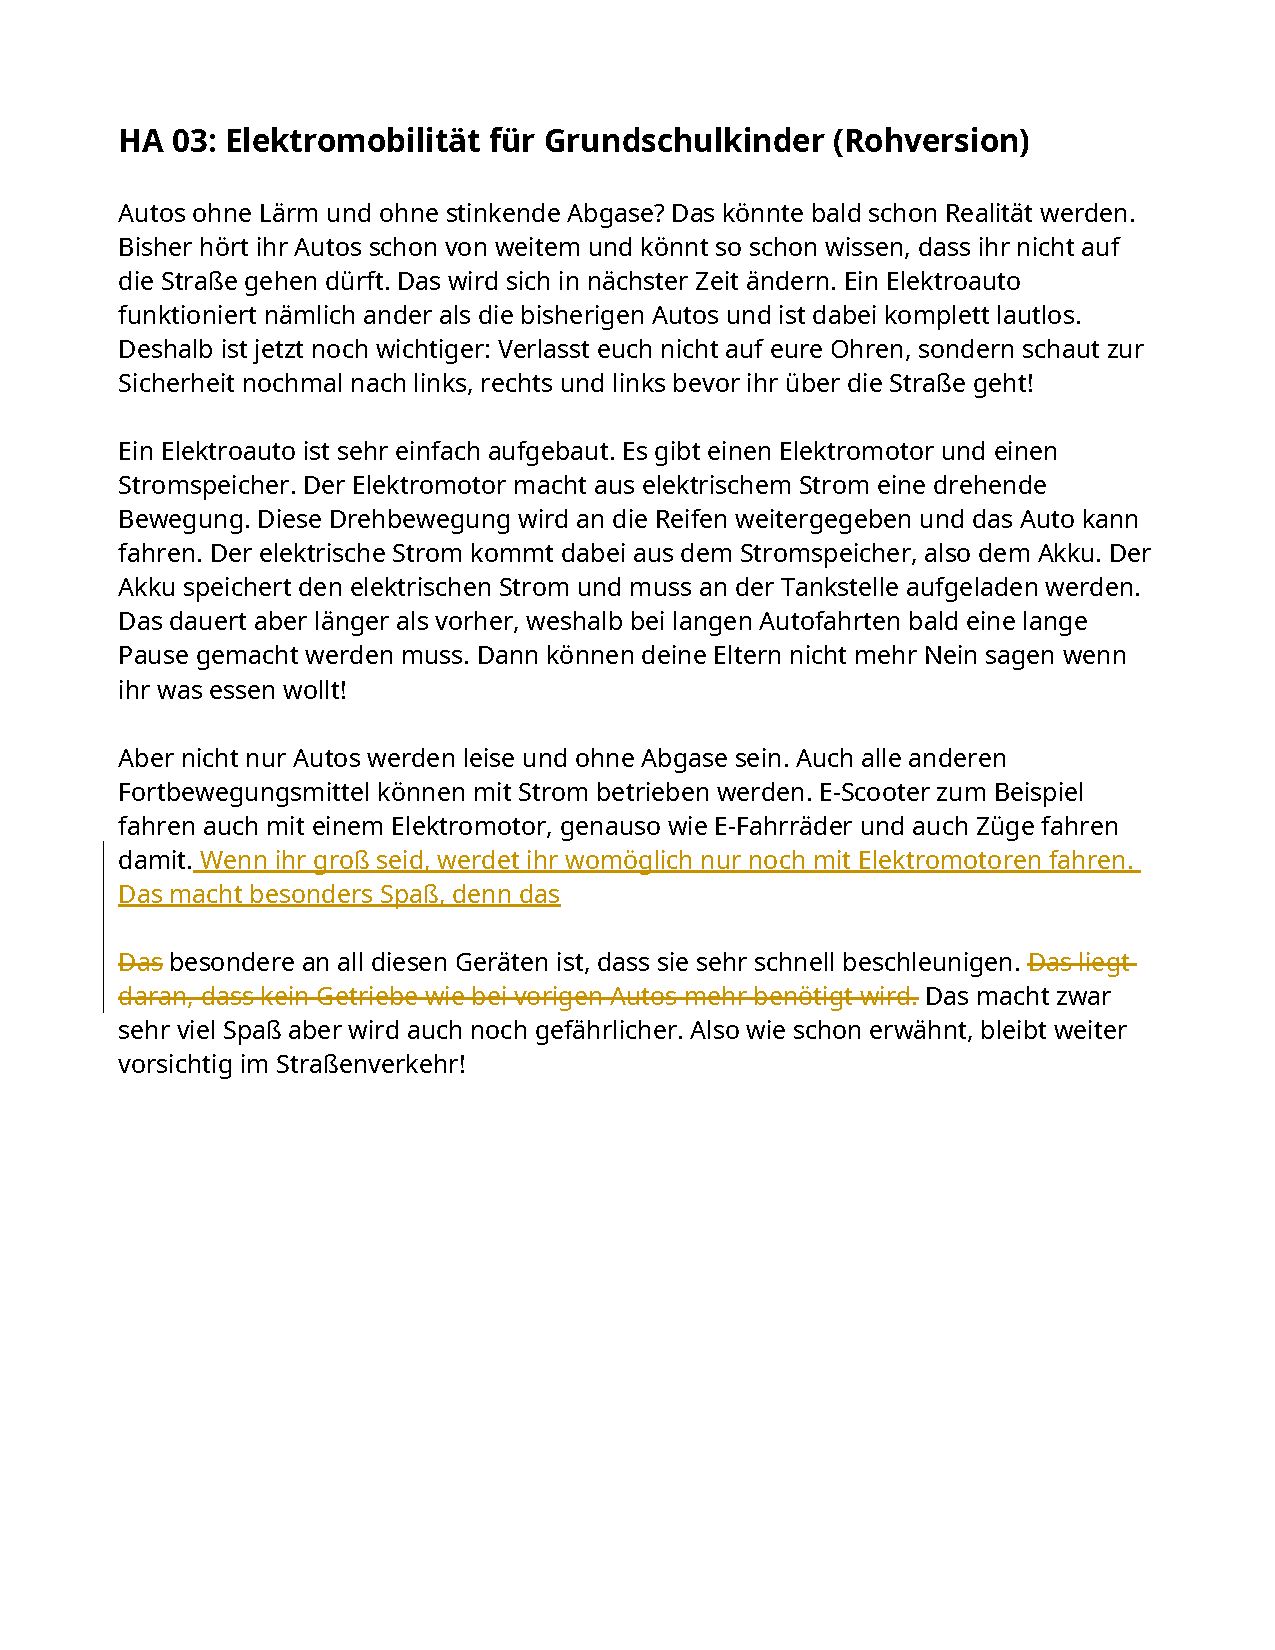
\includepdf[pages=-]{./Hausaufgaben/3_Elektromobilitaet/Elektromobilitaet_Johannes_Rohversion.pdf}

\end{document}
